%%%%%%%%%%%%%%%%%%%%%%%%%%%%%%%%%%%%%%%%%%%%%%%%%%%%%%%%%%%%%%%%%%%%%%%%%%%%
% Section 3: Getting Started
%	This section contains installation instructions for RapidSmith2, and
%	how to test the installation is correct. 
%%%%%%%%%%%%%%%%%%%%%%%%%%%%%%%%%%%%%%%%%%%%%%%%%%%%%%%%%%%%%%%%%%%%%%%%%%%%
\newpage
\section{Getting Started}

\subsection{Installation}

RS2 is available on Github at:
{\color{blue}{\url{https://github.com/byuccl/RapidSmith2}}}.
You can either build RS2 into .class and .jar files for use in any Java
environment, or configure RS2 to work in an IDE (recommended).

\subsubsection{Requirements for Installation and Use}
\begin{itemize}
  \item Windows, Linux or Mac OS X all will work (see additional notes below for
  Mac OS X)
  \item Vivado 2016.2. Later versions of Vivado may work, have not been tested
  yet. Earlier versions will not work.
  \item JDK 1.8 or later
  \item Tincr 
\end{itemize}

Tincr is a companion project
({\color{blue}{\url{https://github.com/byuccl/tincr}}}) which is used for
importing/exporting designs between Vivado and RS2.  For getting started (running the example programs on the provided sample designs) you will not need it installed.
Later, as you  actually start processing your own Vivado designs you will need
to obtain and install it. There are additional dependencies beyond these
required for installation, but they are either provided in the distribution
itself or are automatically retrieved for you as a part of the installation process. 
Examples of these additional dependencies include QT Jambi and the BYU Edif
Tools.
 
\subsubsection{Steps for Installation}

\begin{enumerate}
  \item Clone the RS2 repository at
  {\color{blue}{\url{https://github.com/byuccl/RapidSmith2}}}. If you are not
  familiar with GitHub, you will need to install Git on your computer, and run the
  following command in an open terminal: 
\vspace{-0.07in}
\begin{code}
git clone https://github.com/byuccl/RapidSmith2
\end{code} 
  \noindent This will copy the RS2 repository into a local directory.
  \item Create a new environment variable called RAPIDSMITH\_PATH, and point it
  to your local repository of RS2 that you setup in step (1). This is needed so
  RS2 can find required device files and other items at runtime.
  \item Build the  RS2 project. RS2 is managed using a gradle build system.
  To build the project, navigate to your local repository of RS2 and execute one
  of the following scripts in a terminal:
  \begin{code}
	gradlew build (unix)
	gradlew.bat build (windows)
  \end{code}
  The build process could take a few minutes.
  \item At this point, you have two choices: set up RS2 for use in an IDE, or
  run RS2 from the command line. Both choices are detailed below.
  \paragraph{Running from an IDE} The gradle scripts in RS2 currently support
  setup for both Eclipse and IDEA Java IDEs. This section will detail how to
  setup the Eclipse environment, but similar steps can be taken for IDEA. If
  using Eclipse, it is best to use version Eclipse Neon or later. To create a
  new eclipse project, execute one of the following in a terminal:
  \begin{code}
	gradlew antlr eclipse (unix)       
	gradlew.bat antlr eclipse (windows)
  \end{code}
  Executing these will create an Eclipse \fil{.project} file. After the project
  file has been created, you can import the project into Eclipse by opening
  Eclipse and selecting:
  \begin{code}
	File->Open Projects From File System 
  \end{code}
  and pointing it to your RapidSmith2 local repository. All Java source files
  will be found under \dir{src/main/java}. \pgm{NOTE:} Your RS2 git repository
  should not be put inside your eclipse workspace. It is better to put it
  elsewhere, and then import it into your workspace.
  \paragraph{Building on the Command Line} After step (3) in the installation
  process, gradlew produces everything that you will need to run RS2 from the
  command line. The following directories are created: 
  \begin{itemize}
    \item \fil{build/classes/main}: This folder contains the RS2 class file
    directory tree.
    \item \fil{build/libs}: This folder contains a Jar file of the RS2 class
    files.
    \item \fil{build/distributions}: This folder has both .zip and .tar files
    with contains all Jars needed to run RS2 from the command line. This
    includes a full jar of the RS2 build alond with copies of dependency Jars
    (such as QT-Jambi).
  \end{itemize} 
  After adding the appropriate .class files or Jars to your \texttt{CLASSPATH},
  you should be able to run RS2 tools from the command line. If you make any
  changes to the RS2 code, you will have to rebuild before running the program
  again (Step 3). \pgm{CAUTION:} An obvious thing to try is to mix and match
  developing in Eclipse but then running the resulting apps from the command
  line. Just be aware that Eclipse puts its compiled .class files in very
  different places than where the gradle build process puts its .class and
  .jar files. Make sure you understand that before you try to combine these two
  build/execution methods. Our suggested approach is to choose one or the
  other, but not both.
\end{enumerate}

\subsubsection{Alternative Installation and Use}

RapidSmith2 is also available as a Docker container. To painlessly set up a working RapidSmith2 environment, type:
\vspace{-0.05in}
\begin{code}
docker run -it byuccl/rapidsmith2
\end{code}
\vspace{0.04in}
For more information about Docker, see the \href{https://docs.docker.com/engine/getstarted/}{\color{blue}guide}.

\subsubsection{Additional Notes for Mac OS X Installation}

The instructions above require you to set the \env{RAPIDSMITH\_PATH}
environment variable.  If running from the command line, the environment
variables can be added to your \fil{.bash\_profile} file as in any other
UNIX-like system.  However, if using an IDE such as Eclipse you either need to
define the environment variable for every Run Configuration you create, or you
need to add the \env{RAPIDSMITH\_PATH} definition system-wide in OS X. This can
be done, but how to do so differs based on what OS X version you are running
(and seems to have changed a number of times over the years). Search the web for
instructions for how to do so if you desire. \pgm{Hint}: you will likely have
to edit some \fil{.plist} files.

\subsubsection{Running RS2 Programs}
Some points to keep in mind while configuring and running RS2 programs:
\begin{itemize}
  \item The RS2 code base contains a number of assertions which may be helpful  
  as you are developing code.  These are not enabled by default in Java.  To
  enable them, add \opt{-ea} as a VM argument.  This is highly recommended.
  \item If you are running on a Mac, when running RS2 programs that use Qt  (any
  of the built-in programs like \pgm{DeviceBrowser}) that are GUI-based, you
  will need to supply an extra JVM switch, \opt{-XstartOnFirstThread}.
  \item A common error when running RS2 programs is failing to have your
  \env{RAPIDSMITH\_PATH} defined.  If this is the case when you try to execute a
  program, an \texttt{EnvironmentException} will be thrown telling you that you
  forgot to set the variable.
  \item If you are running on Windows, only a 32-bit QT Jar file is included in
  the RS2 repository. This means that you will need to set your JRE to a 32-bit
  version when running the GUI programs. We are working on updating QT to the
  latest version, so this will no longer be an issue.
  \item For Linux command line usage, the \env{CLASSPATH} environment variable
  must point to both the full (uncompressed) RS2 jar in the \dir{build/distributions}
  folder as well as all the jar files in the \dir{/lib} subdirectory. An example
  \env{CLASSPATH} could look like this:
  \vspace{-0.15in}  \begin{code}
  �  �  � RAPIDSMITH2-SNAPSHOT/*:RAPIDSMITH2-SNAPSHOT/lib/*
  \end{code}
\end{itemize}

\subsubsection{Testing Your Installation}
\noindent At this point you can test your installation by executing the java
\pgm{DeviceBrowser} program: 
\begin{code}
java edu.byu.ece.rapidSmith.device.browser.DeviceBrowser
\end{code} \vspace{0.1in}    

\noindent This can be done either from within Eclipse or from the command line,
depending on how you are running RS2 (if running under OS X be sure to provide the
\opt{-XstartOnFirstThread JVM argument}. If all goes well you should see a
graphical representation showing the details of a physical FPGA device as shown
in \autoref{fig:deviceBrowser}.  You may initially be zoomed far in and might
want to zoom out to see the entire chip layout.

\begin{figure}[H]
\centering
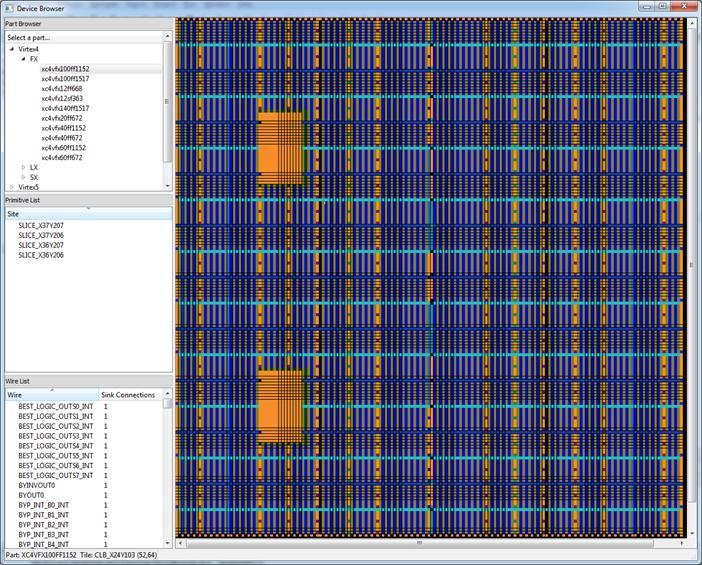
\includegraphics[width=0.8\columnwidth]{deviceBrowser}
\caption{\pgm{DeviceBrowser} Sample Display}
\label{fig:deviceBrowser}
\end{figure}

\subsection{Running Real Designs - An Overview}
This section will lead you through running an entire design from Vivado through
RS2 and back.  In this example you will fully synthesize and implement a
complete design in Vivado and then move it into RS2.  However, later as you gain
experience you may choose to only synthesize  designs before exporting
them to RS2 or you may choose to export and work with Vivado Out-Of-Context
(OOC) Checkpoints.

The steps to be covered include:

\begin{enumerate}
  \item Synthesize, place and route a design in Vivado
  \item  Export the design from Vivado in the form of an RSCP (RapidSmith
  Checkpoint)
  \item Import the RSCP  into RS2
  \item Run some analysis on the design
  \item Export the design from RS2 as a TCP (Tincr Checkpoint)
  \item Import the TCP back into Vivado
\end{enumerate}

In a real CAD flow you would likely do something more interesting
than the analysis in Step 4 above, but this overview is intended to help you
through the Vivado-to-RS2-back-to process so you can get started.

Note: the entire flow requires the installation of Tincr as well as RS2 so if
you skipped the Tincr installation above, go and install it now.

\subsubsection{Synthesize, Place, and Route a Design in Vivado and Then Export
It As a RSCP} If you desire, you may do this step any way you are used to using
Vivado (with or without using the Vivado GUI for example).  In this step, we
will do it using the Vivado Tcl interface.

First, start up Vivado in command line mode.  This can be done using the
``Vivado Tcl Shell'' program item or by executing ``vivado -mode tcl''.  Once
the shell has started up, you may execute the following:
                
\vspace{-0.15in}  \begin{code}
	Vivado\% cd <path to directory containing your HDL files>
	Vivado\% link_design -part xc7a100t-csg324-3
	Vivado\% read_verilog [glob *.v]
	Vivado\% synth_design -top myTopLevelEntityName -flatten_hierarchy full 
	Vivado\% place_design
	Vivado\% route_design
	Vivado\% package require tincr
	Vivado\% tincr::write_rscp myTopLevelEntityName
	Vivado\% close_project
\end{code}
Most of the above commands should be self-explanatory and can be adapted to
compile VHDL or SystemVerilog files.
Importantly,  you must flatten the design hierarchy when running
the synthesis step as shown above.  The result of executing this will be a new
directory which contains the RapidSmith Checkpoint.

As already mentioned, this shows how to create a fully placed and routed design
in Vivado prior to export.  There is no requirement, however, that the design is
either placed or routed prior to export.  You may choose to export it any time
after it has been synthesized.

Finally, note that a set of sample HDL designs are provided in the RS2
distribution and which you could use for your learning.
You can read about them as well as a script which implements a version of the
above compilation steps in Section~\ref{sampledesigns} of this report.  Note
that the compilation script described there expects a particular directory
structure to hold your source files.  Otherwise, the script implements 
essentially what is shown above.

\subsubsection{Import the RSCP into RS2}
Once you have a RSCP you are ready to create a Java program for RS2 that will be
able to import that RSCP into RS2 so you can do something with it.

As described in Section~\ref{examples} of this report (and
Section~\ref{sec:importExportExample} in particular) a sample import/export program
is provided in the RS2 distribution which illustrates how to import
and export designs from RS2.  This program, when run, will read in a
RapidSmith checkpoint (RSCP), walk the resulting data structures and
ten prettyprint the design contents, and then write out the
corresponding Tincr checkpoint.   

You should examine the code for that
program to understand its operation and the subroutine calls that can
be used to do those steps.  The net result from running that program
is to export a Tincr checkpoint, stored in a directory with a ``tcp'' extension.

\subsubsection{Importing a Tincr Checkpoint Back into Vivado}
At this point you can import the resulting Tincr checkpoint back into Vivado. 
Assuming the original RSCP was ``add.rscp'', after running the import/export
example program  you will have a ``add.rscp.tcp'' directory.  After starting
Vivado up in Tcl mode (``vivado -mode tcl'') you can execute the following
commands to import the checkpoint:

\vspace{-0.15in}  \begin{code}
	Vivado\% cd <path to directory containing your add.rscp.tcp directory>
	Vivado\% package require tincr
	Vivado\% tincr::read_tcp add.rscp.tcp
	Vivado\% start_gui
\end{code}

At this point the Vivado GUI will open and you will see that there are cells and
nets associated with this design.  If you want to save the imported design for
later you could also do the following command:

\vspace{-0.15in}  \begin{code}
	Vivado\% write_checkpoint -force add.dcp
\end{code}

You could then later re-load that into Vivado using the following commands from
the Tcl window:

\vspace{-0.15in}  \begin{code}
	Vivado\% link_design -part xc7a100t-csg324-3
	Vivado\% open_checkpoint add.dcp
\end{code}

You will notice that these instructions focus on running Vivado in Tcl mode to
do all the commands given.  The Vivado GUI is then started once the
commands have executed.  Why not just always run in GUI mode since those same
commands could have been typed into the command window in the GUI? It turns out
that running commands such as these while the GUI window is open makes them run
many times slower than if they were run just in Tcl mode.  So, a typical use
case you might find helpful is to always start Vivado in Tcl mode, do the
commands needed to export or import things, and then open the GUI (using
``start\_gui'') and close the GUI (using ``stop\_gui'') as needed.


